% Include at a fixed width: scaling DOWN would push the
% in-figure type below the 9pt floor the artwork guide sets.
\begin{figure}[t]
  \centering
  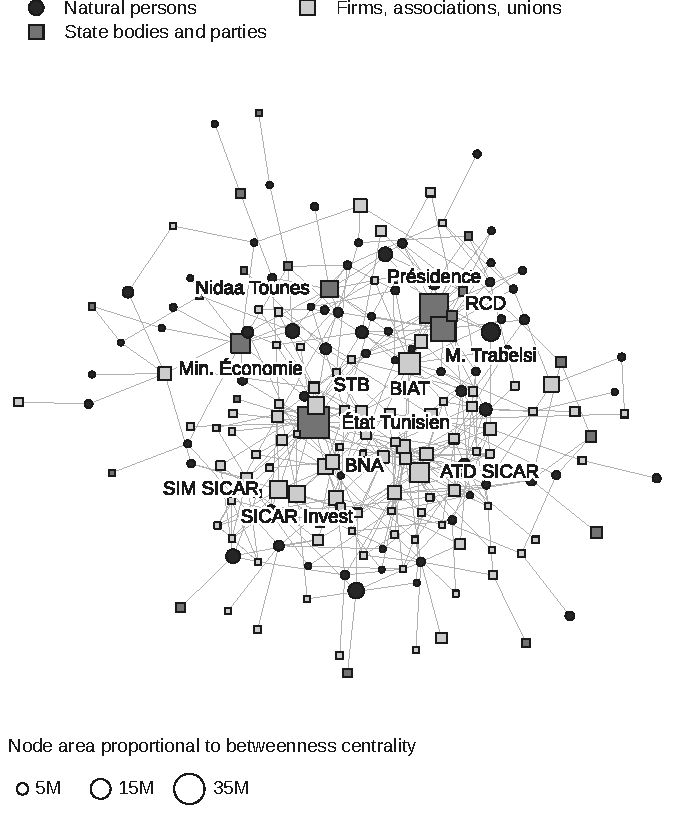
\includegraphics[width=4.5in]{fig15_brokerage_network.pdf}
  \caption{\textbf{The brokerage core of the Tunisian elite network.}
  Node area is proportional to betweenness centrality. The 377
  entities shown, joined by 801 ties, are the giant
  component of the subgraph induced on the 400 highest
  betweenness entities, which together hold 50.3\% of
  all betweenness in the graph. Selection is therefore on
  the quantity the node areas encode; the full network of 23,274 entities
  and 31,457 ties cannot be rendered legibly at page width. Ties are
  undirected and undated, pooling shareholding, board and governing-body
  membership, kinship, party and parliamentary structures, and the seed
  roster, over 1957--2026.
  The composition is 156 natural persons, 31 state bodies and
  parties, and 190 firms, associations and unions. The 10
  highest-brokerage entities are labelled. Abbreviations: Présidence, Présidence de la République; RCD, central committee of the RCD; BIAT, Banque Internationale Arabe de Tunisie; M. Trabelsi, Mohamed Trabelsi; STB, Société Tunisienne de Banque; F. Derbel, Faycel Derbel; Ch. Tuniso-Française, Chambre Tuniso-Française de Commerce et d'Industrie; UBCI, Union Bancaire pour le Commerce et l'Industrie.}
  \label{fig:fig15_brokerage_network}
\end{figure}

% ---------------------------------------------------------------------
% Accessibility description (APSR requires one; WCAG 2.1 AA)
% ---------------------------------------------------------------------
% A node-link diagram of 377 entities connected by
% 801 lines, drawn in greyscale. Circles are natural
% persons, squares are organisations; darker fills are state bodies and
% parties, lighter fills are firms, associations and unions. The area of
% each shape is proportional to its betweenness centrality, so the
% entities that lie on the most shortest paths appear largest. A small
% number of very large nodes, led by État Tunisien,
% sit at the centre of the diagram and connect several otherwise separate
% dense clusters of smaller nodes. A size key at the lower left gives
% reference areas in millions.
